\documentclass[11pt]{article}
%-----------Packeges---------------%
\usepackage{amsmath}
\usepackage{amssymb}
\usepackage{amsfonts}
\usepackage{tocloft}
\usepackage{float}
\usepackage{graphicx}
\usepackage[bookmarks=true]{hyperref}
\usepackage{fancyhdr}


%----------Definition & Theorem----%
\newtheorem{definition}{Definition}[subsection]
\newtheorem{theorem}{Theorem}[subsection]
\newtheorem{proposition}{Proposition}[subsection]
\newtheorem{lemma}{Lemma}[subsection]
\newtheorem{corollary}{Corollary}[subsection]

\usepackage{tikz}
\usetikzlibrary{automata, positioning}
\pagestyle{fancy}
\fancyhead[L]{CS357}
\fancyhead[C]{HW5Q1}
\fancyhead[R]{Lanxiao Bai}
\begin{document}
	\paragraph{Part1}
	
	The graph with fill rank adjacent matrix:
		\begin{figure}[h]
				\begin{center}
					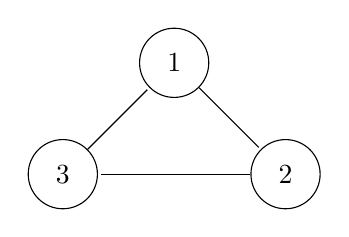
\begin{tikzpicture}[shorten >=1pt,node distance=2cm,on grid,auto]
						\node[state] (1) {$1$};
						\node[state] (2) [below right of=1] {$2$};
						\node[state] (3) [below left of=1] {$3$};
						\path[-]
						(1) edge node {} (2)
						(2) edge node {} (3)
						(3) edge node {} (1);
					\end{tikzpicture}
					\caption{3 node graph with full-rank adjacent matrix}
				\end{center}
			\end{figure}
			
	And its adjacent matrix is
					\[\begin{bmatrix}
						0 & 1 & 1\\
						1 & 0 & 1\\
						1 & 1 & 0
					\end{bmatrix} \]
					
	The graph with rank-deficient adjacent matrix:
		\begin{figure}[h]
				\begin{center}
					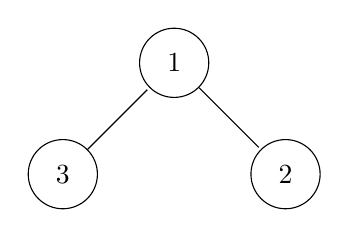
\begin{tikzpicture}[shorten >=1pt,node distance=2cm,on grid,auto]
						\node[state] (1) {$1$};
						\node[state] (2) [below right of=1] {$2$};
						\node[state] (3) [below left of=1] {$3$};
						\path[-]
						(1) edge node {} (2)
						(3) edge node {} (1);
					\end{tikzpicture}
					\caption{3 node graph with rank-deficient adjacent matrix}
				\end{center}
			\end{figure}
	And its adjacent matrix is
					\[\begin{bmatrix}
						0 & 1 & 1\\
						1 & 0 & 0\\
						1 & 0 & 0
					\end{bmatrix} \]
	\paragraph{Part2}
		Define $G = (V, E)$ that $V = \{v_m : m \in \{0, 1, \cdots, n\}\}$ and $E = \{(v_0, v_m) : m \in \{0, 1, \cdots, n\}\}$.
		
	\paragraph{Part3}
		For an arbitrary graph $G$, let $A$ be $G$'s adjacent matrix so $L = D - A$. We notice that for all natural number $m \in [1, n]$, 
			\[\sum_{i = 1}^n l_{mi} = 0\]
			
			then if we scale it with constant $c$, 
			\[\sum_{i = 1}^n cl_{mi} = c0 =0\]
			
			still holds, which means 
			\[[l_{m1}, l_{m2}, \cdots, l_{mn}][c, c, \cdots, c]^T = 0\]
			
			and as a result, 
			\[\mathbf{L}[c, c, \cdots, c]^T = \mathbf{0}\]
			
			Hence, for all $c \in \mathbb{R}$, $\mathbf{v} = c[1, 1, \cdots, 1]$, $\mathbf{Lv} = \mathbf{0}$.
			
			This means that the nullity $\text{Null}(\mathbf{L}) \geq 1$, so by Rank-nullity theorem $\text{Rank}(\mathbf{L}) \leq n - 1$, which means $\mathbf{L}$ is rank-deficient.
	\paragraph{Part4}
		To prove that $\text{Rank}(\mathbf{L}) = n - 1$, we want to rule out the possibility that $\text{Rank}(\mathbf{L}) = n - 1$, which means we want to see that its impossible that $\text{Null}(\mathbf{L}) > 1$.
		
		Suppose $\text{Null}(\mathbf{L}) > 1$, then $\mathbf{w}$ is another solution to equation $\mathbf{Lw = 0}$ that $w \notin \{c[1, 1, \cdots, 1] : c \in \mathbb{R}\}$, and $\text{Rank}([\mathbf{v, w}]) = 2$, then $\mathbf{w} \neq c\mathbf{v}$ for all $c \in \mathbf{R}$.
		
		Let an arbitrary vector $\mathbf{z} = \mathbf{w} - \alpha\mathbf{v}$, that the largest in $\mathbf{w}$ is annihilated. Then consider the structure of $\mathbf{L}$, there is always a diagonal element $\mathbf{L}_{ii}$ that $\mathbf{w}_i = 0$, so
		\[\sum_{i = 1}^n l_{mi} \leq 0\]
		since elements in $-\mathbf{A}$ is nonpositive, the the equality holds only when $\mathbf{z = 0}$. But this is impossible since $\text{Rank}([\mathbf{v, w}]) = 2$.
		
		Hence, we conclude that $\text{Null}(\mathbf{L}) = 1$, and, by Rank-Nullity Theorem, $\text{Rank}(\mathbf{L}) = n - 1$.
\end{document}
